%=====================================================================
% 7  量子力学
% 原文：Section 7. Quantum mechanics（arXiv:2409.03117v1, p. 79--97）
%=====================================================================
\section{量子力学}

\begin{keytakeaways}
\begin{itemize}
  \item \textbf{物理图像：}一维时空（空间维数为零）上的量子场论就是量子力学。把时间解析延拓到虚轴，即作 Wick 转动，虚指数的路径积分便化为实指数的欧氏路径积分；后者有严格的测度论对应（布朗运动），并可反过来用来定义 Minkowski 关联函数。
  \item \textbf{数学工具：}欧氏关联函数并不由测度给出，而是由 Feynman 图级数\emph{定义}：取定函数空间、二次型与各阶张量（顶点），以算子的 Green 函数作传播子，再按图的对称群阶数求和；连通关联函数、配分函数、其对数的生成函数与单粒子不可约有效作用量之间由 Legendre 变换相联系。
  \item \textbf{关键结论：}动量空间的 Feynman 规则把每个连通图的积分重数降为圈数（树图无积分）；欧氏传播子在解析延拓回 Minkowski 号差时给出带无穷小虚部的传播子，其符号由围道绕开极点的方向唯一确定。
  \item \textbf{易错点：}测度归一化（动量空间积分测度的约定）、配分函数本身不可定义而只能定义其比值、无质量情形的零模与红外发散、圆值场按映射度分扇区以及由此产生的 theta 函数结构，都是本章的易错之处，正文中已逐处点明。
\end{itemize}
\end{keytakeaways}

\bigskip
\noindent\rule{\textwidth}{0.6pt}
\bigskip

迄今为止，我们讨论的是时空维数为零的量子场论（开个玩笑说，可以认为空间的维数是 $-1$）。本节将更接近真实的物理：我们考虑一维时空，也就是空间的维数为 $0$。这并不意味着我们要研究零维空间中的运动（那实在是一件憾事），而只是意味着我们只考察点状的量子客体（粒子），而不考察延展的量子客体（场）。换言之，我们将进入量子力学的领域。

\subsection{量子力学中的路径积分}
设 $U(q)$ 是实轴上的光滑函数（即势能）。我们假定 $U(0)=0$、$U'(0)=0$、$U''(0)=m^2$，其中 $m>0$。

\begin{remark} 在量子场论中，势能里的参数 $m$ 称为\emph{质量}参数。更确切地说，在经典力学中它的含义是振动的频率 $\omega$。然而在量子理论中，按照 Einstein，频率与能量等同（$E=\hbar \omega/2\pi$）；而在相对论理论中，能量又与质量等同（同样按照 Einstein，$E=mc^2$）。
\end{remark} 

我们要建立量子粒子在势场 $U(q)$ 中运动的量子理论。按照先前的讨论，这意味着我们要赋予下述归一化关联函数以意义并对其求值：
$$
\langle q(t_1) \ldots q(t_n)\rangle:=
\frac{\int q(t_1) \ldots q(t_n)e^{\frac{iS(q)}{\hbar}}Dq}{\int e^{\frac{iS(q)}{\hbar}}Dq}, 
$$
其中 $S(q)=\int {\mathcal L}(q)dt$，而 ${\mathcal L}(q)=\frac{\dot{q}^2}{2}-U(q)$。

正如我们已经讨论过的，当 $\hbar$ 为正数时，这类积分无法用测度论严格处理；因此我们只在“微扰论意义下”定义这些路径积分，亦即把它们定义成 $\hbar$ 的形式级数。

在给出这一（完全严格的）定义之前，我们先解释其背后的动机。需要提醒读者：这一解释是启发式的，其中包含在数学上并不严格的步骤（或者用物理学家的说法，是“形式”的步骤）。

\subsection{Wick 转动}

在第 1 章中我们讨论过带有虚指数的路径积分（量子力学），也讨论过带有实指数的路径积分（布朗运动）。如果 $\hbar$ 是一个数，那么带有虚指数的积分无法按测度论定义。因此，人们转而研究带有实指数的积分（它可以被严格定义），然后再施行一个特殊的解析延拓手续，称为\emph{Wick 转动}。

在我们的形式化框架中（$\hbar$ 是形式参数），实情形与虚情形的积分其实都可以定义。尽管如此，实情形毕竟稍容易一些，因此 Wick 转动仍然有用。此外，Wick 转动在概念上极为重要。所以，尽管它在技术上并非必需，我们仍先在这里引入 Wick 转动。

具体说来，我们把 $\langle q(t_1)...q(t_n)\rangle$ 记为 $\G^M_n(t_1,...,t_n)$，并在 $\G^M_n(t_1,...,t_n)$ 的公式中“形式地”作变量替换 $\tau=it$。令 $q(t):=q_*(\tau)$。于是，注意到 $d\tau=idt$、$\frac{dq}{dt}=i\frac{dq_*}{d\tau}$，我们得到
$$
\G^M_n(t_1,...,t_n)=
\frac{\int q_*(\tau_1) \ldots q_*(\tau_n)e^{-\frac{1}{\hbar}\int (\frac{1}{2}
(\frac{dq_*}{d\tau})^2+U(q_*))d\tau}Dq_*}{\int e^{-\frac{1}{\hbar}\int (\frac{1}{2}
(\frac{dq_*}{d\tau})^2+U(q_*))d\tau}Dq_*}. 
$$
这表明
$$
\G^M_n(t_1,...,t_n)=\G^E_n(it_1,...,it_n),
$$
其中
$$
\G^E_n(t_1,...,t_n):=
\frac{\int q(t_1) \ldots q(t_n)e^{-\frac{S_E(q)}{\hbar}}Dq}{\int e^{-\frac{S_E(q)}{\hbar}}Dq}. 
$$
其中 $S_E(q)=\int {\mathcal L}_E(q)d\tau$，且 ${\mathcal L}_E(q)=\frac{\dot{q}^2}{2}+U(q)$
（也就是说，把 ${\mathcal L}$ 中的 $U$ 换成 $-U$ 便得到 ${\mathcal L}_E$）。

这一操作当然没有严格意义，但它启发了下述定义。

\begin{definition}
函数 $\G^M_n(t_1,...,t_n)$（$t_i\in \Bbb R$）是函数 $\G^E_n(\tau_1,...,\tau_n)$ 沿路径
$\theta\mapsto e^{i\theta}(t_1,...,t_n)$（$0\le \theta\le \pi/2$）从点
$(t_1,...,t_n)$ 到点 $(it_1,...,it_n)$ 的解析延拓。
\end{definition}

当然，只有当我们定义了函数 $\G^E_n(t_1,...,t_n)$ 并证明它具有所需的解析延拓时，这个定义才有意义。这一点将在下文完成。

\begin{remark} （关于术语。）函数 $\G^M_n(t_1,...,t_n)$ 称为 \emph{Minkowski}（时间有序）关联函数，而函数
$\G^E_n(t_1,...,t_n)$ 称为\emph{欧氏}关联函数（记号即由此而来）。这一术语将在后面讨论相对论性场论时解释。

 从现在起，我们主要处理欧氏关联函数，因此在不会引起混淆时将省略上标 $E$。
\end{remark}

% [Tutor Note: 定义 7.2 的“解析延拓”之所以有意义，是因为每个 $F_\Gamma$ 都是初等函数的有限组合：在固定的时间序区域 $t_{\sigma(1)}\ge\cdots\ge t_{\sigma(n)}$ 内，可把 $G(t_i-t_j)=e^{-m|t_i-t_j|}/(2m)$ 中的绝对值去掉，内点积分化为 $\int s^r e^{-\alpha s}ds$ 一类的初等积分，故 $\G_n$ 在该区域是 $t_i^r e^{a t_i}$ 型函数的有限线性组合。于是可先在每个开区域上定义解析函数，再核对它们在边界上拼接一致，从而得到沿 $t\mapsto e^{i\theta}t$ 的解析延拓。原文在此只作断言而未给细节；若要严格化，需逐图核对区域边界上的拼接，并说明所得函数沿四分之一圆周的路径有界（这正是 $\theta\mapsto e^{i\theta}$ 而非其他路径的原因）。此外，$m>0$ 保证欧氏传播子指数衰减，这是全部收敛性的来源；Minkowski 侧的无穷小虚部 $i\varepsilon$ 正是这一旋转留下的痕迹。]

\subsection{欧氏关联函数的定义}

现在我们的任务是定义欧氏关联函数 $\G_n(t_1,...,t_n)$。
我们的策略如下（这一策略也将用于场论）。回想一下：若所涉积分是有限维的，那么由 Feynman 定理，关联函数关于 $\hbar$ 的展开就由各 Feynman 图振幅之和给出。因此，在无穷维情形下，我们直接把对 Feynman 图的求和作为关联函数的\emph{定义}。

更具体地说，由于对 $U$ 所加的条件，作用量泛函中没有 $q$ 的常数项与线性项，于是关联函数 $\G_n(t_1,...,t_n)$ 应由下述求和给出：
\begin{equation}\label{defcor}
\G_n(t_1,...,t_n)=
\sum_{\Gamma\in G_{\ge 3}^*(n)}\frac{\hbar^{b(\Gamma)}}{|{\rm Aut}(\Gamma)|}
F_\Gamma(\ell_1, \ldots ,\ell_n),
\end{equation}
其中 $G_{\ge 3}^*(n)$ 的定义见注 \ref{G3*}。
因此，我们需要在目前的情形下赋予振幅 $F_\Gamma$ 以意义（也就是给出定义）。为此，需要定义以下对象。

1. 空间 $V$。

2. $V$ 上的形式 $B$，它定义 $V^*$ 上的 $B^{-1}$。

3. 作用量中非二次项对应的张量。

4. 余向量 $\ell_i$。

如何自然地定义这些对象是清楚的。具体说来，$V$ 应取为 $\Bbb R$ 上满足一定衰减条件的函数空间。
$V$ 的选取方式很多，且不影响最终结果；例如一个良好的选择（也是我们将采用的）是 $\Bbb R$ 上紧支光滑函数构成的空间 $C^\infty_0(\Bbb R)$。
于是 $V^*$ 就是 $\Bbb R$ 上的分布空间。
注意 $V$ 上配有内积 $(f,g)=\int_{\Bbb R}f(x)g(x)dx$。

与有限维情形类比，形式 $B$ 应取为作用量二次部分的两倍。换言之，
$$
B(q,q)=\int(\dot{q}^2+m^2q^2)dt=(Aq,q),
$$ 
其中 $A$ 是算子
$$
A=-\frac{d^2}{dt^2}+m^2.
$$ 
这意味着 $B^{-1}(f,f)=(A^{-1}f,f)$。

算子 $A^{-1}$ 是积分算子，其核为
$$
K(x,y)=G(x-y),
$$ 
其中
$G(x)$ 是 $A$ 的 Green 函数，亦即下述微分方程的基本解（在无穷远处衰减）：
$$
(AG)(x)=\delta(x).
$$ 
直接计算可得
$$
G(x)=\frac{e^{-m|x|}}{2m}.
$$ 
（因此 $B^{-1}$ 实际上并非在整个 $V^*$ 上有定义，而是在 $V^*$ 的一个稠密子空间上有定义）。

\begin{remark} 这里我们已经看到 Wick 转动的用处。具体说来，$A$ 的谱（按通常意义，把它看作 $L^2(\Bbb R)$ 上的自伴无界算子）是 $[m^2,+\infty)$，故它可逆且逆算子有界。然而，若不作 Wick 转动，我们面对的将是算子 $A'=-\frac{d^2}{dt^2}-m^2$，其谱为 $[-m^2,+\infty)$，即含有 $0$，因此该算子没有有界逆。
\end{remark}

为使作用量中的三次及更高次项成为张量，考虑 $U$ 在 $x=0$ 处的（渐近）Taylor 级数展开：
$$
U(x)=\frac{m^2x^2}{2}-\sum_{n\ge 3}\frac{g_nx^n}{n!}.
$$ 
这表明作用量中三次及更高次项具有形式
$$
B_r(q,q,,...,q)=\int q^r(t)dt.
$$ 
% [Tutor Note: 原文此处写作 $B_r(q,q,,...,q)$，多了一个逗号，应为 $B_r(q,\ldots,q)$，系笔误（译文按规范保留原式）。按第 3 章的约定，$B_r$ 是 $r$ 元对称张量：它由线性化作用量中的 $\int q^r$ 项给出，与 $r$ 个变元缩并即得 $B_r(q,\ldots,q)=\int q^r(t)dt$。另注意记号上 $B$ 既表示二次型又表示 $B_r$ 一族张量，原文依赖上下文区分。]
于是 $B_r(q_1,...,q_r)$ 是 $(S^rV)^*$ 中的元素，由分布 $\delta_{t_1=...=t_r}$（对角线的 delta 函数）给出。

最后，泛函 $\ell_i$ 由 $\ell_i(q)=q(t_i)$ 给出，故 $\ell_i=\delta(t-t_i)$。

由此得到下述定义图 $\Gamma$ 振幅的 Feynman 规则。

1. 给 $\Gamma$ 的第 $i$ 个外顶点赋以数 $t_i$。

2. 给 $\Gamma$ 的每个内顶点 $j$ 赋以一个变量 $s_j$。

3. 在连接顶点 $j$ 与 $j'$ 的每条内边上写 Green 函数 $G(s_j-s_{j'})$。

4. 在连接 $i$ 与 $j$ 的每条外边上写 $G(t_i-s_j)$。

5. 在连接 $i$ 与 $i'$ 的每条外边上写 $G(t_i-t_{i'})$。

6. 令 $G_\Gamma(\bold t,\bold s)$ 为这些函数的乘积。

7. 令 $F_\Gamma(\ell_1,...,\ell_n):=\prod_j g_{v(j)}\int G_\Gamma(\bold t,\bold
s)d\bold s$，其中 $v(j)$ 是 $j$ 的价数。

现在我们终于可以给出下述定义。

\begin{definition}
函数 $\G_n(t_1,...,t_n)$ 由公式 \eqref{defcor} 定义。
\end{definition}

\begin{remark} 注意定义 $F_\Gamma$ 的积分是收敛的，因为被积函数在无穷远处总是指数衰减的。然而，关键在于我们只考虑不含“没有外顶点的连通分支”的图；例如，若 $\Gamma$ 只有一个四价顶点，并由两条圈与自身相连（图 21），那么振幅积分中就会出现 $\int_{\Bbb R}G(0)^2ds$，它显然是发散的。
\end{remark}

按此定义，函数 $\G_n(t_1,...,t_n)$ 是关于 $\hbar$ 的 Laurent 级数，其系数是 $t_1,...,t_n$ 的对称函数，由一些显式的（且收敛的）有限维积分的线性组合给出。
此外，容易看出这些积分实际上可以用初等函数算出，也就是说（在区域 $t_1\ge...\ge t_n$ 内）它们是形如 $t_i^re^{at_i}$ 的函数的乘积的线性组合。
这就蕴含了 Wick 转动手续中所需解析延拓的存在性。

\begin{figure}[htbp]
  \centering
  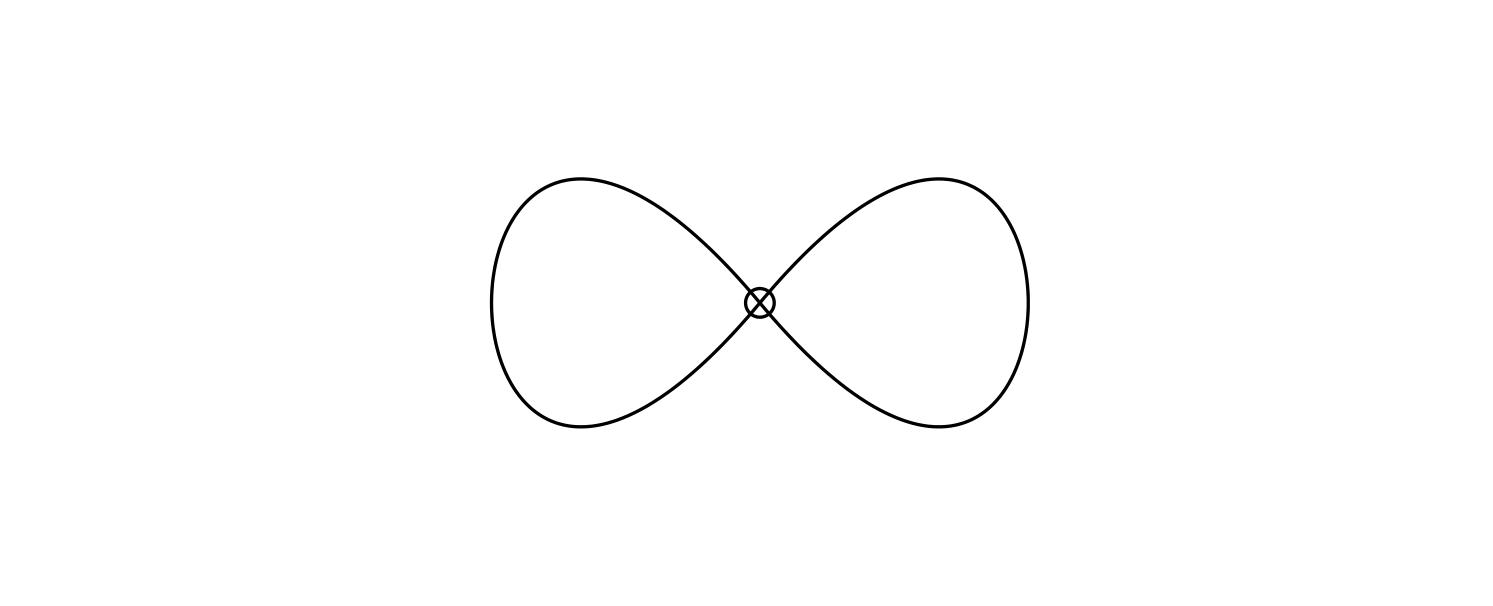
\includegraphics[width=6.32cm]{figures/fig-21.png}
  \caption{（原文无图题）\figorig{84}{21}}
  \label{fig:21}
\end{figure}

\begin{remark} 与有限维情形一样，给出这一定义的另一种方案是假定 $g_i$ 都是形式参数。此时 $\hbar$ 可以取数值，例如 $\hbar=1$，而函数 $\G_n$ 将是 $g_3,g_4,...$ 的一个良定义的幂级数。
\end{remark}

作为例子，考虑自由的有质量理论，即\emph{谐振子}：$U(q)=\frac{m^2q^2}{2}$。此时没有内顶点，因此得到

\begin{proposition} （Wick 定理）当 $n$ 为奇数时 $\G_n(t_1,...,t_n)=0$，并且
$$
\G_{2k}(t_1,...,t_{2k})=\hbar^{k}\sum_{\sigma\in \Pi_k}\prod_{i\in
  \lbrace{1,...,2k
\rbrace}/\sigma}G(t_i-t_{\sigma(i)}).
$$
\end{proposition}

特别地，$\G_2(t_1,t_2)=\hbar G(t_1-t_2)$。
换言之，$\G_2(t_1,t_2)$ 就是（正比于）Green 函数。受此启发，物理学家常把量子场论的一切关联函数都称为 \emph{Green 函数}。

\begin{figure}[htbp]
  \centering
  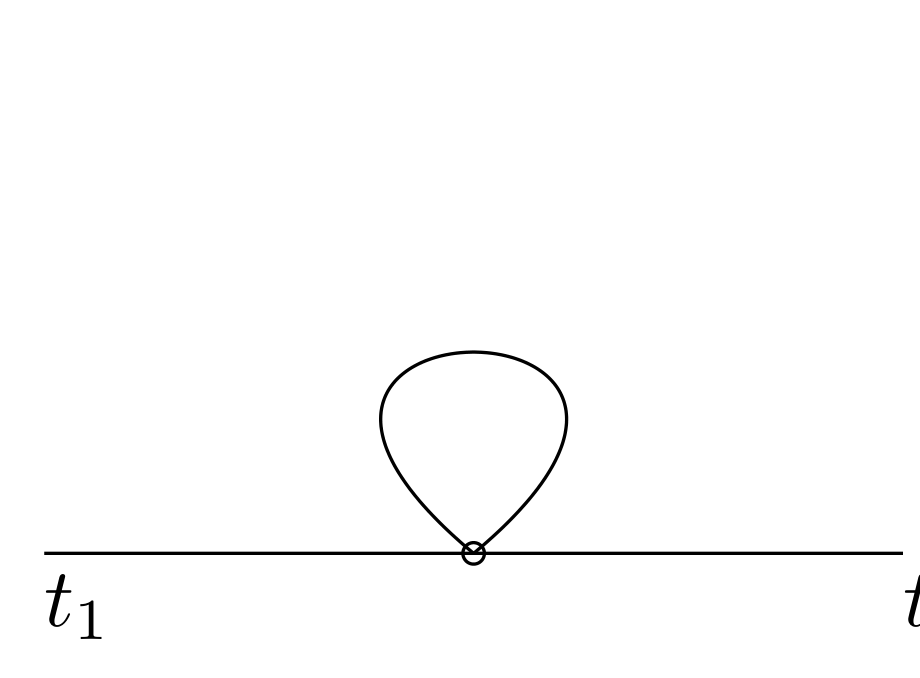
\includegraphics[width=3.89cm]{figures/fig-22.png}
  \caption{（原文无图题）\figorig{85}{22}}
  \label{fig:22}
\end{figure}

\begin{example} 考虑势能 $U(q)=\frac{m^2q^2}{2}-\frac{gq^4}{24}$，
并令 $\hbar=1$。
此时我们来计算两点关联函数模 $g^2$。
换言之，需要算出该函数中 $g$ 的系数。
因此要考虑带两条外边和一个内顶点的 Feynman 图。
这样的图 $\Gamma$ 是唯一的：它由一条边以及附着在其中点的一个圈构成（图 22）。该图的自同构群为 $\Bbb Z/2$。此图的振幅为
$$
F_\Gamma=g\int_{\Bbb R}G(s,t_1)G(s,t_2)G(s,s)ds=
\frac{g}{8m^3}\int_{\Bbb R}e^{-m(|s-t_1|+|s-t_2|)}ds.
$$
由于对 $t_1$ 与 $t_2$ 的对称性，不妨设 $t_1\ge t_2$。把积分拆成三个积分之和，分别取在 $(-\infty,t_2],[t_2,t_1]$ 与 $[t_1,\infty)$ 上，我们得到：
$$
F_\Gamma=
\frac{g}{8m^3}\left(2\int_0^\infty e^{-m(2s+|t_1-t_2|)}ds+|t_1-t_2|e^{-m|t_1-t_2|}\right)=
$$
$$
\frac{g}{8m^4}e^{-m|t_1-t_2|}(1+m|t_1-t_2|).
$$
因此
$$
\G_2(t_1,t_2)=\widetilde{G}(t_1-t_2),
$$
其中
$$
\widetilde{G}(t):=\tfrac{1}{2m}e^{-m|t|}+\tfrac{g}{16m^4}e^{-m|t|}(1+
m|t|)+O(g^2).
$$
这一表达式称为两点函数的\emph{单圈近似}，因为它来自零圈与单圈 Feynman 图。
\end{example} 

\begin{remark} 这里我们考虑的是单个一维粒子的量子力学。
不过，一切都可毫无困难地推广到 $n$ 维粒子或粒子系统的情形（亦即推广为对一维向量值函数而非标量函数的路径积分）。
事实上，若 $q$ 取值于欧氏空间 $V$，则拉格朗日量的二次部分具有形式 $\frac{1}{2}(\dot{q}^2-M(q))$，其中 $M$ 是 $V$ 上的正定二次型。把 $M$ 对角化后，可以假定拉格朗日量的二次部分形如 $\frac{1}{2}\sum_i(\dot{q_i}^2-m_i^2q_i^2)$，这对应于一组相互独立的谐振子。于是在量子理论中传播子将是对角矩阵，其对角元为 $\frac{e^{-m_i|t-s|}}{2m_i}$，而关联函数可按通常的 Feynman 图手续定义。
\end{remark}

\subsection{连通关联函数}

设 $\G^{c}_n(t_1,...,t_n)$ 为\emph{连通关联（或 Green）函数}，其定义为：与 $\G_n(t_1,...,t_n)$ 相同的振幅之和，但只对连通 Feynman 图求和。显然
$$
\G_n(t_1,...,t_n)=\sum_{\lbrace{1,...,n\rbrace}=S_1\sqcup...\sqcup
  S_k} 
\prod \G^c_{|S_i|}(t_j; j\in S_i).
$$
例如，$\G_2(t_1,t_2)=\G_2^c(t_1,t_2)+\G_1^c(t_1)\G_1^c(t_2)$，等等。因此，只要知道连通关联函数，就足以知道关联函数。

\begin{example}\label{harosc} 在自由理论（$U=\frac{m^2q^2}{2}$，即谐振子）中，除 $\G_2$ 以外的一切连通 Green 函数都为零。
\end{example} 

\begin{figure}[htbp]
  \centering
  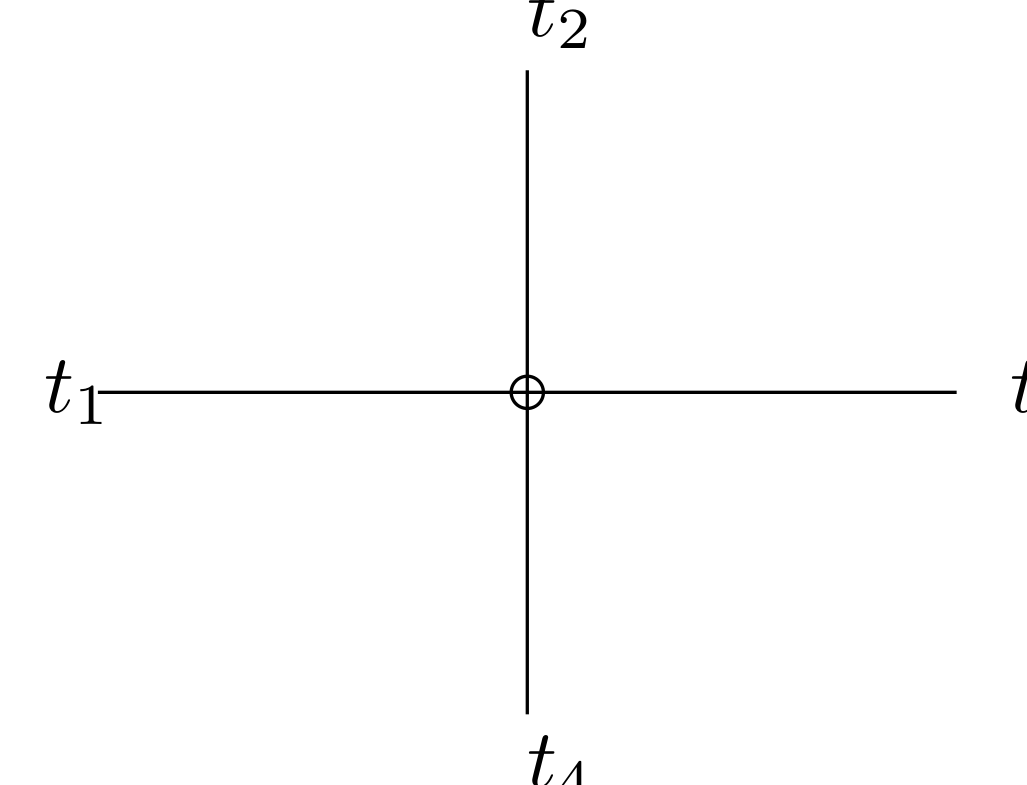
\includegraphics[width=4.35cm]{figures/fig-23.png}
  \caption{（原文无图题）\figorig{86}{23}}
  \label{fig:23}
\end{figure}

\begin{example} 我们来计算上述四次势 $U=\frac{m^2q^2}{2}-\frac{gq^4}{4}$ 所对应理论中的连通四点函数，模 $g^2$。这意味着应当计算带一个内顶点和四条外边的连通 Feynman 图的贡献。这样的图 $\Gamma$ 是唯一的——就是十字形图（带一个内顶点），见图 23。此图没有非平凡自同构。于是
$$
\G_4^c(t_1,t_2,t_3,t_4)=g\int_{\Bbb R}
G(t_1-s)G(t_2-s)G(t_3-s)G(t_4-s)ds+O(g^2).
$$
这个积分可以用初等方法算出；我们把它留作习题。
\end{example} 

\subsection{聚类性质} 
注意 Green 函数 $G(t)$ 在无穷远处趋于零。
这蕴含自由理论关联函数的如下\emph{聚类性质}：
$$
\lim_{z\to \infty} \G_{n}(t_1,...,t_r,t_{r+1}+z,...,t_n+z)=
\G_r(t_1,...,t_r)\G_{n-r}(t_{r+1}...t_n).
$$
此外，容易证明在有相互作用的理论（即带势能的理论）中，就 $\hbar$ 的每一阶而言同样成立（请自行验证！）。聚类性质可以更简洁地写成等式
$$
\lim_{z\to \infty} \G_{n}^c(t_1,...,t_r,t_{r+1}+z,...,t_n+z)=0.
$$
这一性质有物理解释：彼此相距遥远的过程几乎是统计独立的。因此，它可以看作量子场论“具有物理意义”的一个必要条件。

\begin{remark} 尽管如此，确实存在不满足聚类性质、但从物理与数学角度看都很有趣的理论（例如所谓的\emph{拓扑量子场论}；见下文第 \ref{fqm} 小节）。
\end{remark} 

\subsection{配分函数}
设 $J(t)dt$ 是实轴上具有紧支集的测度。考虑“带外源 $J$ 的配分函数”，它是一个形式表达式
$$
Z(J)=\int e^{\frac{-S_E(q) +(J,q)}{\hbar}}Dq.
$$ 
于是我们有形式等式
$$
\frac{Z(J)}{Z(0)}=\sum_n \frac{\hbar^{-n}}{n!}\int_{\Bbb R^n}
\G_n(t_1,...,t_n)J(t_1)...J(t_n)dt_1...dt_n,
$$
与先前一样，我们将把这个等式用作 $Z(J)/Z(0)$ 的定义。于是，知道 $Z(J)/Z(0)$ 等价于知道全部 Green 函数（换言之，$Z(J)/Z(0)$ 是它们的生成函数）。此外，与有限维情形一样，我们有

\begin{proposition} 有
$$
W(J):=\log \frac{Z(J)}{Z(0)}=
\sum_n \frac{\hbar^{-n}}{n!}\int\G_n^c(t_1,...,t_n)J(t_1)...J(t_n)dt_1...dt_n
$$
（亦即 $W$ 是连通 Green 函数的生成函数）。
\end{proposition}

% [Tutor Note: 这里的关键是“归一化”。无穷维路径积分测度 $Dq$ 的归一化因子是无穷大，$Z(0)=\int e^{-S_E/\hbar}Dq$ 本身并不存在（相当于真空图振幅不能求和，参见前文关于“无外顶点分支”的注），可定义的只是比值 $Z(J)/Z(0)$；等价地，$W=\log(Z(J)/Z(0))$ 的展开只含连通图，真空图自动消去。原文坚持写 $Z(J)/Z(0)$ 而非 $Z(J)$，正是为了避开这一乘性无穷大。注意下文在时间紧化到圆上之后，常数函数的积分变为有限，$Z(0)$ 才成为可定义的对象。]

此命题的证明与有限维情形相同。

\begin{remark} 命题的陈述等价于上一小节给出的通常 Green 函数与连通 Green 函数之间的关系。
\end{remark} 

\begin{remark} 我们只能定义那些所有连通分支都至少含一个一价顶点的图的振幅（见上文），这意味着我们实际上既不能定义 $Z(0)$，也不能定义 $Z(J)$，而只能定义它们的比值 $Z(J)/Z(0)$。
\end{remark} 

与有限维情形一样，我们有展开
$$
W(J)=\hbar^{-1}W_0(J)+W_1(J)+\hbar W_2(J)+...,
$$
其中 $W_j$ 是 $j$ 圈贡献（特别地，$W_0$ 由对树的求和给出）。此外，与有限维情形类似，我们对 $W_0$ 与 $W_1$ 有显式公式。

\begin{proposition} 有
$$
W_0(J)=-S_E(q_J)+(q_J,J), 
$$
其中 $q_J$ 是泛函 $S_E^J(q):=S_E(q)-(q,J)$ 的极值点，且在无穷远处衰减。此外，
$$
W_1(J)=-\frac{1}{2}\log \det L_J,
$$ 其中 $L_J$ 是 $V$ 上的线性算子，满足
$$
d^2S_E^J(q_J)(f_1,f_2)=d^2S_E^0(0)(L_Jf_1,f_2).
$$
\end{proposition}

此命题的证明尤其需要说明 $q_J$ 是良定义的，并且 $\det L_J$ 存在。它类似于第 \ref{treepar} 小节中给出的有限维情形同一结果的证明（确切地说，我们当时只证明了零圈情形；但单圈情形的证明是类似的）。因此我们不给出该证明，而宁可用一个例子来说明这一结论。

\begin{example} 设 $U$ 为上文的四次势 $\frac{m^2q^2}{2}+\frac{gq^4}{2}$（为方便起见我们改变了四次项的正负号与归一化），并令 $J(t)=a\delta(t)$。
此时
$$
S_E^J(q)=\int(\tfrac{\dot{q}^2}{2}+U(q))dt-aq(0).
$$ 
欧拉–拉格朗日 方程具有形式
$$
\ddot{q}=m^2q+2gq^3-a\delta(t).
$$
于是函数 $q_J$ 由非线性微分方程
$$
\ddot{q}=m^2q+2gq^3
$$ 
在 $(-\infty,0]$ 与 $[0,\infty)$ 上的两个解 $q_+,q_-$ 连续拼接而成，且在 $0$ 处导数跃变为 $-a$。

我们要求 $q_+,q_-$ 在无穷远处衰减，故它们必须是零能量的解：
$$
E=\frac{\dot{q_\pm}^2}{2}-U(q_\pm)=0.
$$
因此，按 Newton 方程解的标准公式，它们由下述等式确定：
$$
t-t_{\pm}=\int\frac{dq}{\sqrt{2U(q)}}=\int \frac{dq}{mq\sqrt{1+\frac{gq^2}
{m^2}}}=
\frac{1}{2m}\log\frac{\sqrt{1+\frac{gq^2}{m^2}}-1}
{\sqrt{1+\frac{gq^2}{m^2}}+1}.
$$
经过计算可得
$$
q_J(t)=\frac{2mg^{-\frac{1}{2}}}{C^{-1}e^{m|t|}-Ce^{-m|t|}},
$$
其中 $C$ 是方程
$$
\frac{C(1+C^2)}{(1-C^2)^2}=\frac{ag^{\frac{1}{2}}}{4m^2}
$$
的解，它由 $a$ 的幂级数给出且常数项为零。由此用初等方法（但稍嫌冗长）可以算出 $W_0=-S_E^J(q_J)$。

现在，算子 $L_J$ 由下述公式给出
$$
L_J=1+\frac{gA^{-1}\circ q_J(t)^2}{2},
$$ 
其中 $A=-\frac{d^2}{dt^2}+m^2$。因此 $\det L_J$ 是有意义的。事实上，算子 $A^{-1}\circ q_J(t)^2$ 是积分算子，其核为
$$
K_J(x,y):=\frac{e^{-m|x-y|}q_J(y)^2}{2m},
$$ 
它在无穷远处指数衰减；因此算子 $1+\frac{gA^{-1}\circ q_J(t)^2}{2}$ 的行列式是良定义的。
\end{example}

\begin{remark} 在这些计算中，$g, a$ 是形式变量，但只要 $ga^2+m^2>0$，上述计算实际上对这些变量的实数值也成立。
\end{remark} 

\subsection{单粒子不可约 Green 函数}

用 $\G^{1PI}_n(t_1,...,t_n)$ 表示\emph{单粒子不可约（1PI）Green 函数}，亦即与通常 Green 函数相同的振幅之和，但只对单粒子不可约 Feynman 图求和。再定义\emph{截腿}（amputated）单粒子不可约 Green 函数：$\G^{1PIa}_n:=A^{\otimes n}\G^{1PI}_n$
（它由同样的振幅之和定义，只是在每条外边上不写 $G(t_i-s_j)$，而写 $\delta(t_i-s_j)$）。

设 $S_{\rm eff}(q)$ 是 $\G_n^{1PIa}$ 的生成函数，即
$$
S_{\rm eff}(q)=\sum_n\frac{\hbar^{-n}}{n!}\int
\G^{1PIa}_n(t_1,...,t_n)
q(t_1)...q(t_n)dt_1...dt_n.
$$

\begin{proposition} 函数 $W(J)=\log(Z(J)/Z(0))$
是 $S_{\rm eff}(q)$ 的 Legendre 变换，即它等于
$-S_{\rm eff}(\widetilde q_J)+(J,\widetilde q_J)$，其中 $\widetilde q_J$ 是
$-S_{\rm eff}(q)+(J,q)$ 的极值点，且在无穷远处衰减。
\end{proposition}

此命题的证明与有限维情形相同。该命题表明，
为了知道 Green 函数，“只需”知道
截腿单粒子不可约 Green 函数
（通常 Green 函数的生成函数可由 1PI Green 函数的生成函数经
Legendre 变换与指数化重构出来）。
这是个好消息，因为 1PI 图比一般的连通图少得多。

\subsection{动量空间积分}

我们已经看到，Feynman 图的振幅由维数等于内顶点个数的空间上的积分给出。这有时并不方便，
因为即便是树图，这类积分也可能相当复杂。然而，一旦转到 Fourier 变换，
Feynman 积分就会简化，特别是连通图的积分重数等于圈数（于是树图根本不需要积分）。

具体做法如下。
我们不用时间变量 $t$，而考虑其对偶的能量变量 $E$。具有紧支集的函数
$q(t)$ 将用它的 Fourier 变换 $\widehat q(E)$ 代替。
于是由 Plancherel 定理，对实函数
$q_1,q_2$ 有
$$
(q_1,q_2)=\int_{\Bbb R}q_1(t)q_2(t)dt=\int_{\Bbb R} \widehat q_1(E)\overline{\widehat q_2(E)}dE=
\int_{\Bbb R} \widehat q_1(E)\widehat q_2(-E)dE.
$$
这表明传播子由下式给出：
$$
B^{-1}(f,f)=\int_{\Bbb R} \frac{1}{E^2+m^2}\widehat f(E)\widehat f(-E)dE.
$$
位于 $k$ 价顶点处的顶点张量原为 $\delta_{s_1=...=s_k}$，因此将被替换为 $\delta_{Q_1+...+Q_k=0}$，其中 $Q_i$ 是与 $s_i$ 对偶的变量。

\begin{remark} （关于术语）物理学家把时间变量 $t_i,s_j$ 称为\emph{位置变量}，
把能量变量 $E_i,Q_k$ 称为\emph{动量变量}，因为在相对论力学中
（这正是我们研究场论时所处的框架），时间与位置之间、能量与动量之间并无区别
（这是 Lorentz 群作用的结果）。
\end{remark}

这表明，对于给定的、带 $n$ 个外顶点的连通 Feynman 图 $\Gamma$，
其“动量空间”Feynman 规则如下。

1. 给图 $\Gamma$ 定向，使所有外边的方向朝内。

2. 给每条外线（外边）赋变量 $E_i$，给每条内线（内边）赋变量 $Q_j$。这些变量满足
“第一 Kirchhoff 定律”的线性方程：
在每个内顶点处，流入边对应的变量之和等于流出边对应的变量之和。
设 $Y(\bold E)$ 为这些方程的解 $\bold Q$ 构成的空间（它依赖于 $\Gamma$，但我们不显式写出这种依赖）。容易证明，该空间非空仅当 $\sum_i E_i=0$ 时成立，而在这种情况下 $\dim Y(\bold E)$ 等于 $\Gamma$ 的圈数（请证明这一点！）。

3. 在每条外边上写 $\frac{1}{E_i^2+m^2}$，在每条内边上写 $\frac{1}{Q_k^2+m^2}$。
令 $\phi_\Gamma(\bold E,\bold Q)$ 为这些函数的乘积。

4. 把 $\Gamma$ 的\emph{动量空间振幅}定义为分布 $\widehat F_\Gamma(\bold E):$
$$
\widehat F_\Gamma(E_1,...,E_n)=
\prod_jg_{v(j)}
\int_{Y(\bold E)}\phi_\Gamma(\bold E,\bold Q)d\bold Q\cdot \delta(E_1+...+E_n)d\bold E,
$$
它支撑在超平面 $\sum_i E_i=0$ 上。
显然该分布不依赖于 $\Gamma$ 的定向。

\begin{remark} 这里我们须规定空间 $Y(\bold E)$ 上（平移不变的）Lebesgue 测度  $d\bold Q$ 
的归一化。其定义方式是：使 $Y(\bold E)/Y_{\Bbb Z}(0)$ 的体积为 $1$，其中 $Y_{\Bbb  Z}(0)$ 是 $Y(0)$ 中整数元素的集合。因此，若 $T\subset \Gamma$ 是一棵生成树，则在 $Y(\bold E)$ 的坐标 $\lbrace Q_e,e\notin T\rbrace$ 下，
有 $d\bold Q=\prod_{e\notin T}dQ_e$。
 \end{remark} 

% [Tutor Note: 这里的归一化约定最容易出错：$d\bold Q$ 并不是由 $\Bbb R^{\#\text{内边}}$ 上的坐标体积直接诱导的，而是要求基本胞腔 $Y(\bold E)/Y_{\Bbb Z}(0)$ 的体积为 $1$（把整数格点的基本域归一到单位体积）；等价地，沿生成树 $T$ 取独立圈变量时有 $d\bold Q=\prod_{e\notin T}dQ_e$，此即“第一 Kirchhoff 定律”把圈变量与树变量分开的标准做法。原文的 Fourier 变换采用不含 $2\pi$ 的约定（见 $1/(E^2+m^2)=\int G(t)e^{iEt}dt$ 与 $G(t)=e^{-m|t|}/(2m)$），即把 $2\pi$ 吸收进了测度；与常见的 $1/(2\pi)\int$ 约定相比，每个圈积分少一个 $(2\pi)^{-1}$ 因子，与场论章节的约定核对时必须统一。]

现在我们有

\begin{proposition}
函数 $F_\Gamma(\delta_{t_1},...,\delta_{t_n})$ 的 Fourier 变换是
$\widehat F_\Gamma(E_1,...,E_n)$。
因此，连通 Green 函数的 Fourier 变换为
\begin{equation}\label{defcor1}
\widehat\G_n^c(E_1,...,E_n)=
\sum_{\Gamma\in G_{\ge 3}^*(n)}\frac{\hbar^{b(\Gamma)}}{|{\rm Aut}(\Gamma)|}
\widehat F_\Gamma(E_1, \ldots, E_n).
\end{equation}
\end{proposition}

此命题的证明是直接的。

为说明该命题，考虑一个例子。

\begin{example}
四次势的连通四点函数模 $g^2$ 在动量空间中形如：
$$
\widehat \G_4^c(E_1,E_2,E_3,E_4)=
g\prod_{i=1}^4\frac{1}{E_i^2+m^2}\delta(\sum_i E_i)d\bold E+O(g^2).
$$
\end{example}

\begin{figure}[htbp]
  \centering
  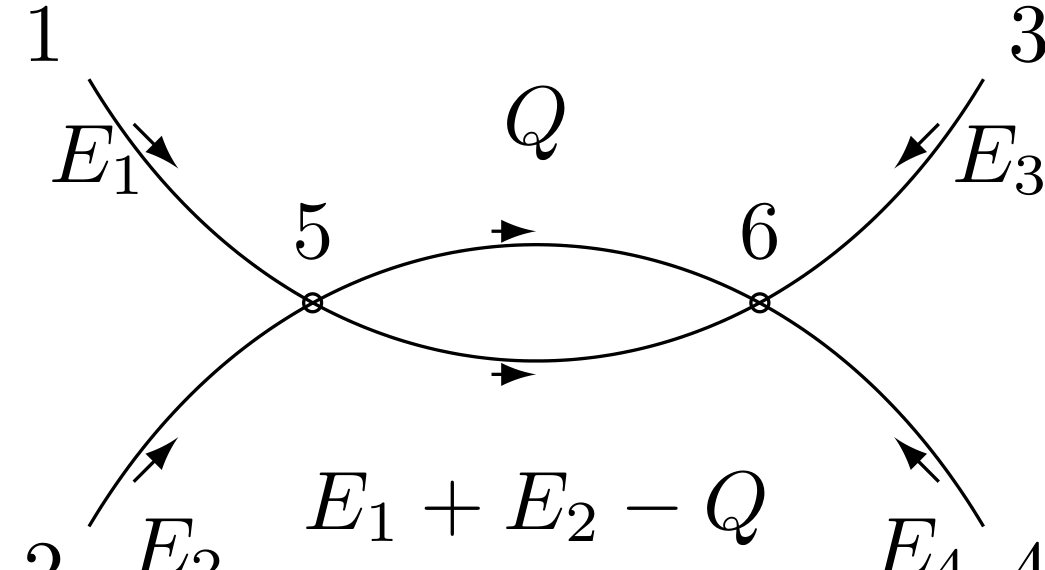
\includegraphics[width=4.42cm]{figures/fig-24.png}
  \caption{（原文无图题）\figorig{92}{24}}
  \label{fig:24}
\end{figure}

\begin{example} 我们来计算同一问题中的 1PI 四点函数，但现在模 $g^3$。因此，除上述项之外，还需算出 $g^2$ 系数，它来自单圈图。这样的图共有三个，彼此相差外边的置换。其中一个图如下：它有外顶点 $1,2,3,4$ 和内顶点 $5,6$，使得 $1,2$ 连接到 $5$，$3,4$ 连接到 $6$，而 $5$ 与 $6$ 由两条边相连（图 24）。此图的对称群为 $\Bbb Z/2$，故其贡献为
$$
\frac{g^2}{2}\left(\int_{\Bbb R}\frac{dQ}{(Q^2+m^2)((E_1+E_2-Q)^2+m^2)}\right)
\prod_{i=1}^4\frac{1}{E_i^2+m^2}\delta(\sum_i E_i)d\bold E.
$$
其中的积分容易算出，例如用留数法。这给出
$$
\widehat \G_4^c(E_1,E_2,E_3,E_4)=
$$
$$
g\prod_{i=1}^4\frac{1}{E_i^2+m^2}
\left(1+\frac{\pi
  g}{m}\sum_{i=2}^4\frac{1}{(E_1+E_i)^2+4m^2}\right)\delta(\sum_i E_i)d\bold E+
O(g^3)
$$
（该式关于 $E_1,E_2,E_3,E_4$ 是对称的，因为当 $\sum_i E_i=0$ 时，对互不相同的 $i,j,k,\ell$ 有
$(E_i+E_j)^2=(E_k+E_\ell)^2$）。
\end{example}

\subsection{动量空间中的 Wick 转动}

为了得到量子力学的关联函数，我们应在欧氏框架下算出它们之后，再把它们 Wick 转动回 Minkowski 框架。我们现在就在动量空间的 Feynman 积分层面上做这件事。（在位置空间做也可以，但就今后的需要而言，在动量空间做更有启发性，因为我们稍后要讨论的高维场论中，动量空间表示更为方便。）

考虑欧氏传播子
$$
\frac{1}{E^2+m^2}=\int_{\Bbb R} G(t)e^{iEt}dt,
$$
其中 $G$ 是 Green 函数。
当我们解析延拓回 Minkowski 框架时，必须在关联函数中把时间变量 $t$ 换成 $e^{i\theta}t$，其中 $\theta$ 从 $0$ 变到 $\frac{\pi}{2}$。特别地，Green 函数 $G(t)$ 必须换成 $G(e^{i\theta}t)$。因此我们必须考虑
$$
\int_{\Bbb R} G(e^{i\theta}t)e^{iEt}dt=
e^{-i\theta} \int_{\Bbb R} G(t)e^{ie^{-i\theta}Et}dt=
\frac{e^{-i\theta}}{e^{-2i\theta}E^2+m^2}.
$$
当 $\theta\to \frac{\pi}{2}$ 时，该函数（作为分布）趋于函数
$\lim_{\varepsilon\to
0+}\frac{i}{E^2-m^2+i\varepsilon}$。
为简洁起见，通常省略极限号，把这个分布写成 $\frac{i}{E^2-m^2+i\varepsilon}$。

由此可见，为了在 Minkowski 框架下计算动量空间中的关联函数，我们应使用与欧氏框架相同的 Feynman 规则，只需把置于边上的传播子换成
$$
\frac{i}{E^2-m^2+i\varepsilon}.
$$
例如，图 24 所示图的贡献为
\scriptsize
$$
-\frac{g^2}{2}\left(\int_{\Bbb R}\frac{dQ}{(Q^2-m^2+i\varepsilon)
((E_1+E_2-Q)^2-m^2+i\varepsilon)}\right)
\prod_{j=1}^4\frac{1}{E_j^2-m^2+i\varepsilon}\delta(\sum_i E_j)d\bold E.
$$
\normalsize

\subsection{圆上的量子力学} 

（至少在数学上）考虑把时间轴换成长度为 $L$ 的圆周情形的欧氏量子力学路径积分是合理的，即 $t\in \Bbb R/L\Bbb Z$（这对应于势场中的一个布朗粒子被条件限制为在给定时间 $L$ 内回到原位置）。
此时理论不变，只是 Green 函数 $G(t)$ 被换成方程 $(-\frac{d^2}{dt^2}+m^2)f=\delta(t)$ 在圆上的周期解 $G_L(t)$。该解具有形式
\begin{equation}\label{glformula} 
G_L(t)=\sum_{k\in \Bbb
  Z}G(t-kL)=\frac{e^{-m(t-\frac{L}{2})}+e^{-m(\frac{L}{2}-t)}}{2m(e^{\frac{mL}{2}}-e^{-\frac{mL}{2}})},\ 0\le t\le L.
\end{equation} 
我们注意到，在圆周情形下，没有外边的图不再引起麻烦（因为常数函数在圆上的积分是收敛的），因此不仅可以定义关联函数（即 $Z(J)/Z(0)$），还可以定义 $Z(0)$ 本身。具体说来，设
$$
U(q)=\frac{m^2q^2}{2}+\sum_{n\ge 3}\frac{g_nq^n}{n!},
$$ 
并令 $m^2=m_0^2+g_2$（其中 $g_i$ 是形式参数）。
于是比值 $Z_{m_0,\bold
  g,L}(0)/Z_{m_0,0,L}(0)$ 是有意义的
（其中 $Z_{m,\bold g,L}(0)$ 表示在指定参数值下的配分函数；此后将省略自变量 $0$）。

事实上，这个比值由下述公式定义：
$$
\frac{Z_{m_0,\bold g,L}}{Z_{m_0,0,L}}=
\sum_{\Gamma\in G_{\ge 2}(0)}\frac{\hbar^{b(\Gamma)}}{|{\rm Aut}(\Gamma)|}
F_\Gamma
$$
（其中 $G_{\ge 2}(0)$ 是没有外顶点、且所有顶点价数 $\ge 2$ 的 Feynman 图之集），而这是一个良定义的表达式。

在情形
$$
g_2=a,\ g_3=g_4=...=0.
$$ 
下计算这一表达式是有启发性的。
此时只有二价顶点，故仅有的连通 Feynman 图是 $N$ 边形，它们都是单圈的。
因此
$$
\log \frac{Z_{m_0,\bold g,L}}{Z_{m_0,0,L}}=
W_1=-\frac{1}{2}\log \det M,
$$
其中
$$
M=1+a(-\tfrac{d^2}{dt^2}+m_0^2)^{-1}.
$$ 
这个行列式可以通过考察本征值来计算。具体说来，$-\frac{d^2}{dt^2}+m_0^2$ 在空间 $C^\infty(\Bbb R/L\Bbb Z)$ 中的本征函数是 $e^{\frac{2\pi int}{L}}$，本征值为 $\frac{4\pi^2n^2}{L^2}+m_0^2$。
于是
$$
\det M=\prod_{n\in \Bbb
  Z}\left(1+\frac{a}{\frac{4\pi^2n^2}{L^2}+m_0^2}\right).
$$
因此，利用 欧拉乘积公式
$$
\sinh(z)=z\prod_{n\ge 1} \left(1+\frac{z^2}{\pi^2n^2}\right),
$$
我们得到
$$
\frac{Z_{m_0,\bold g,L}}{Z_{m_0,0,L}}=
\frac{\sinh(\frac{m_0L}{2})}{\sinh(\frac{mL}{2})}.
$$
（请用对 Feynman 图的求和来复核这一结果！）

\begin{remark} 更通俗地说，我们看到 $U=\frac{m^2q^2}{2}$ 的理论的配分函数 $Z$ 具有形式
$\frac{C}{\sinh(\frac{mL}{2})}$，其中 $C$ 是可以任选的常数。
此后我们取 $C=\frac{1}{2}$；稍后（见例 \ref{benchoi}）会看到为什么这一选择更可取。
\end{remark}

\subsection{无质量情形} 
现在考虑无质量情形，$m=0$。此时传播子应由算子 $-\frac{d^2}{dt^2}$ 求逆得到，亦即它应是核为 $G(t-s)$ 的积分算子，其中 $G(t)$ 是满足微分方程
$$
-G''(t)=\delta(t).
$$ 
的偶函数。
这样的解构成一个单参数族：
$$
G(t)=-\frac{1}{2}|t|+C.
$$ 

利用这个函数（无论 $C$ 如何选取），都可以按 Wick 公式定义自由理论的关联函数。

注意函数 $G$ 在无穷远处不衰减。因此这一理论不满足聚类性质（亦即不是“具有物理意义的”）。

在定义相应的相互作用理论（即带非二次势的理论）时也会遇到困难，因为定义 Feynman 图振幅的积分将会发散。这类发散称为\emph{红外发散}，其起因是被积函数在大时间处不衰减（或者说，在动量空间中它在低频处不正则）。

\subsection{圆值量子力学}
现在考虑拉格朗日量相同、但 $q(t)$ 取值于半径为 $r$ 的圆周 $\Bbb R/2\pi r\Bbb Z$ 的理论（即“sigma 模型”）。至少经典地可以这样做，因为拉格朗日量 $\frac{\dot{q}^2}{2}$ 在此情形下有意义。

我们来定义相应的量子理论。
与线值情形的根本区别在于：既然 $q(t)$ 是圆值的，我们就不应再考虑通常的关联函数
$\langle q(t_1)...q(t_n)\rangle$，而应考虑指数函数的关联函数
$\langle e^{\frac{ip_1q(t_1)}{r}}...e^{\frac{ip_nq(t_n)}{r}}\rangle$，其中 $p_j$ 为整数。它们应由路径积分
\begin{equation}\label{expon}
\int e^{\frac{ip_1q(t_1)}{r}}...e^{\frac{ip_nq(t_n)}{r}}e^{-\frac{S(q)}{\hbar}}Dq,
\end{equation}
定义，其中 $S(q):=\frac{1}{2}\int \dot{q}^2dt$，并约定 $\int e^{-\frac{S(q)}{\hbar}}Dq$ 等于 $1$。
注意只需考虑 $\sum_j p_j=0$ 的情形，否则沿圆周的平移群在被积函数上非平凡地作用，从而在任何合理的定义下该积分都应为零。

现在我们来定义积分 (\ref{expon})。
由于该积分在沿目标圆周的平移下不变，我们不妨设想积分是在 $q:\Bbb R\to \Bbb R$ 且 $q(0)=0$ 上进行的。
下面利用有限维类比。
按照这一类比，通过配方我们将得到
$$
\int e^{\frac{ip_1q(t_1)}{r}}...e^{\frac{ip_nq(t_n)}{r}}e^{-\frac{S(q)}{\hbar}}Dq=
e^{-\frac{\hbar}{2r^2} B^{-1}(\sum_j p_jq(t_j),\sum_j p_jq(t_j))}=
$$
$$
e^{-\frac{\hbar}{2r^2}\sum_{j,\ell} p_\ell p_j G(t_\ell-t_j)}=
e^{\frac{\hbar}{2r^2}\sum_{\ell<j} p_\ell p_j|t_\ell-t_j|},
$$
其中 $B(q,q):=\int \dot{q}^2dt$。
因此，自然地把关联函数定义为
$$
\langle e^{\frac{ip_1q(t_1)}{r}}...e^{\frac{ip_nq(t_k)}{r}}\rangle
=e^{\frac{\hbar}{2r^2}\sum_{\ell<j} p_\ell p_j|t_l-t_j|}.
$$
我们注意到，这一理论与线值情形不同，它\emph{确实}满足聚类性质。事实上，
若 $\sum p_j=0$（如我们所假定的），则
（假定 $t_1\ge t_2\ge...\ge t_n$）有
$$
\sum_{\ell<j}p_\ell p_j(t_\ell-t_j)=
\sum_{j=1}^{n-1}(t_j-t_{j+1})(p_{j+1}+...+p_n)(p_1+...+p_j)=
$$
$$
-\sum_j (t_j-t_{j+1})(p_1+...+p_j)^2,
$$ 
于是聚类性质可由 $(p_1+...+p_j)^2\ge 0$ 推出。

\subsection{圆上的无质量量子力学} 

现在考虑拉格朗日量为 $\frac{\dot{q}^2}{2}$、$q$ 是长度为 $L$ 的圆周上的函数的理论。此时，
按照 Feynman 的通行手法，
我们必须在圆 $\Bbb
R/L\Bbb Z$ 上求算子 $-\frac{d^2}{dt^2}$ 的逆，或等价地解微分方程
$-G''(t)=\delta(t)$。这里遇到了麻烦：
算子 $-\frac{d^2}{dt^2}$ 不可逆，因为它有本征函数 $1$、本征值 $0$；相应地，所讨论的微分方程无解，因为 $\int G''dt$
必须为零，故 $-G''(t)$ 不可能等于 $\delta(t)$
（可以说，指数中的二次型是退化的，
因此高斯积分变得没有意义）。
这个问题可以用下述“杀掉零模”的技巧解决。
具体说来，我们在空间
$\lbrace{q\in C^\infty(\Bbb R/L\Bbb Z): 
\int qdt=0\rbrace}$ 上求算子 $-\frac{d^2}{dt^2}$ 的逆（这可以解释为
在这个余维一的子空间上积分，二次型在其上非退化）。这意味着要求解微分方程
$-G''(t)=\delta(t)-\frac{1}{L}$，并满足 $\int Gdt=0$。
这样的解确实是唯一的，它等于
\begin{equation}\label{greefu} 
G(t)=\frac{(t-\frac{L}{2})^2}{2L}-\frac{L}{24},
\end{equation}
$t\in [0,L]$。于是例如
$\langle q(0)^2\rangle=\frac{L}{12}$。 

更高阶的关联函数按通常方式定义。
此外，可以用标准的 Feynman 图手续定义带任意势的理论。

\subsection{圆上的圆值量子力学} 
最后，考虑同一理论的圆值版本。于是积分变量是映射 $q: \Bbb R/L\Bbb
Z\to \Bbb R/2\pi r\Bbb Z$。这样就出现了新特征——
映射按映射度分成不同的同伦类。我们先考虑对映射度为零的映射积分。
此时应按 $t\in \Bbb
R$ 的情形同样论证，并作如下定义：
$$
\langle e^{\frac{ip_1q(t_1)}{r}}...e^{\frac{ip_nq(t_n)}{r}}\rangle_0:=
e^{-\frac{\hbar}{2r^2}\sum_{\ell,j}p_\ell p_j G(t_\ell-t_j)},
$$
其中 $\sum_j p_j=0$。
（这里下标 $0$ 表示映射度为零的映射）。
假定 $0\le t_1,...,t_n\le L$，利用 \eqref{greefu} 作简短计算可得
$$
\langle e^{\frac{ip_1q(t_1)}{r}}...e^{\frac{ip_nq(t_n)}{r}}\rangle_0
=e^{\frac{\hbar}{2r^2}(\sum_{\ell<j} p_\ell p_j |t_\ell-t_j|+\frac{(\sum_j p_jt_j)^2}{L})}
$$
（当 $L\to \infty$ 时第二项消失，从而回到直线上的答案）。

然而，更为自然的做法（我们稍后就会看到）是对所有映射 $q$ 积分，而不只对映射度为零的映射积分。具体说来，设 $N$ 为整数。
则所有映射度为 $N$ 的映射都具有形式
$q(t)+\frac{2\pi rNt}{L}$，其中 $q$ 是映射度为零的映射。因此，若要对映射度为
$N$ 的映射积分，就应计算与映射度为零时相同的积分，
但作平移 $q\mapsto q+\frac{2\pi r Nt}{L}$。
然而容易看出，这一平移只是把被积函数乘上因子 $e^{\frac{2\pi iN}{L}\sum_j
p_jt_j-\frac{2\pi^2r^2N^2}{\hbar L}}$。因此，对所有映射的积分应由下述公式定义：
$$
\langle e^{\frac{ip_1q(t_1)}{r}}...e^{\frac{ip_nq(t_n)}{r}}\rangle=
$$
\begin{equation}\label{thetform}
e^{\frac{\hbar}{2r^2}(\sum_{l<j} p_\ell p_j |t_\ell-t_j|+\frac{(\sum p_jt_j)^2}{L})}
\frac{\sum_{N\in \Bbb Z}e^{\frac{2\pi iN}{L}\sum_j
p_jt_j-\frac{2\pi^2r^2N^2}{\hbar L}}}
{\sum_{N\in \Bbb Z}e^{-\frac{2\pi^2r^2N^2}{\hbar L}}}.
\end{equation}
引入椭圆 theta 函数
$$
\theta(u,T):=\sum_{N\in \Bbb Z}e^{2\pi iuN-\pi TN^2}.
$$
于是对 $L\ge  t_1\ge...\ge t_n\ge 0$，公式 \eqref{thetform} 
可以改写为
\begin{equation}\label{thetaf}
\langle e^{\frac{ip_1q(t_1)}{r}}...e^{\frac{ip_nq(t_n)}{r}}\rangle
=
e^{\frac{\hbar}{2r^2} (\sum_j (t_{j}-t_{j+1})(p_1+...+p_j)^2+\frac{(\sum_j
p_jt_j)^2}{L})}
\frac{\theta(\frac{\sum_j p_jt_j}{L},\frac{2\pi r^2}{\hbar L})}
{\theta(0,\frac{2\pi r^2}{\hbar L})}.
\end{equation}

% [Tutor Note: 这里按映射度分层求和是本章最值得注意的“拓扑”结构：每一层（映射度为 $N$）的积分与零度积分只差一个显式的指数因子，它来自指数函数在 $q\mapsto q+\frac{2\pi rNt}{L}$ 下的平移；因此对所有映射的积分等于零度积分乘以（theta 函数之比）。所引入的 $\theta(u,T)=\sum_N e^{2\pi iuN-\pi TN^2}$ 正是 Jacobi 第三 theta 函数 $\vartheta_3(u\,|\,iT)$：它的 $N$ 求和可用 Poisson 求和改写为对偶的求和，这正是第 13 章环面配分函数的模不变性与 T 对偶的雏形。注意 $T=\frac{2\pi r^2}{\hbar L}$，$L\to\infty$ 对应 $T\to 0$，此时只有 $N=0$ 项存活，与“直线上只保留零度映射”完全一致；$t_i$ 的排序 $L\ge t_1\ge\cdots\ge t_n\ge0$ 只是把 $|t_\ell-t_j|$ 分段写成求和（与前面聚类性质的计算同一手法）。]

\begin{exercise} 对势能为 $U(q):=\frac{m^2q^2}{2}-\frac{gq^4}{4!}$ 的量子粒子，
在动量空间中计算其单粒子不可约两点函数，模 $g^3$，取 $\hbar=1$。
（我们已在位置空间算过模 $g^2$ 的情形）。
\end{exercise}

\begin{exercise} 设 $U(q):=\frac{m^2q^2}{2}-\frac{gq^3}{3}$。

（i）计算一点函数
${\mathcal G}_1(t)$ 的首项（关于 $g$）。

（ii）计算连通两点函数，模 $g^3$。
\end{exercise} 

\begin{exercise} 
 考虑势能 $U(x):=\frac{m^2\sinh^2(gx)}{2g^2}$。
 当 $J(t)=a\delta(t)$ 时，尽可能显式地给出 $W_0(J)$
（即 $\log(Z(J)/Z(0))$ 的树部分）的公式。
\end{exercise} 

\bigskip
\noindent\rule{\textwidth}{0.6pt}
% [Tutor Note: 本章小结——这一章把路径积分从“形式记号”提升为可操作的定义：先用 Wick 转动把问题搬到欧氏号差，再以 Feynman 图级数定义欧氏关联函数，从而完全绕开无穷维测度；随后证明这些图积分由初等函数组合而成，故解析延拓存在，回到 Minkowski 侧即得带 $i\varepsilon$ 的传播子。三个反复出现的陷阱值得记牢：(1) 归一化——只有比值 $Z(J)/Z(0)$ 可定义，动量空间的 $d\bold Q$ 要按格点的基本域归一，Fourier 变换采用无 $2\pi$ 的约定；(2) 无质量时传播子不衰减，导致聚类性质失效并产生红外发散，圆上还需先处理零模（杀掉常数模、减去 $1/L$）；(3) 时间紧化到圆上会出现按映射度分层的拓扑扇区，圆值场的关联函数由 theta 函数给出，这是第 13 章二维共形场论与 T 对偶的出发点。]

